\documentclass{article}

\usepackage{amsmath, amsfonts, amsthm} 
\usepackage{listings}
\usepackage{graphicx}
\usepackage{float}
\usepackage{subfigure}
\usepackage{geometry}

\geometry{
	paper=a4paper, 
	top=2.5cm,
	bottom=2.5cm, 
	left=2.5cm, 
	right=3cm,
	headsep=0.75cm, 
}
\title{ME424 HW4}
\author{Zhuang Yulun 11811126}
\date{\today}

\begin{document}

\maketitle

\section{}
\subsection{}
The system is asymptotically stable if and only if all eigenvalues of A satisfiles $\left|\lambda_i\right|<1$
\\
Since
$
\lambda=
\begin{bmatrix}
    0.9\\1\\1
\end{bmatrix}
$
,eigenvalues of A are not all less than 1, matrix A is not asymptotically stable.
\subsection{}
$H(z)=C(zI-A)^{-1}B+D$\\
The system is BIBO stable if and only if the poles of every entry in $H(z)$ lies inside the unit circle.
\\

$$
(zI-A)^{-1}=
\begin{bmatrix}
    \frac{1}{z-0.9}&0&\frac{1}{(z-0.9)(z-1)}\\
    0&\frac{1}{z-1}&0\\
    0&0&\frac{1}{z-1}
\end{bmatrix}
$$\\
Choose
$
B=
\begin{bmatrix}
    1\\-1\\-1
\end{bmatrix}
$
and
$
C=
\begin{bmatrix}
    1&1&-1
\end{bmatrix}
$
, such that $H(z)=\frac{1}{z-0.9}$ and the pole of $H(z)$ is $0.9<1$.
\section{}
\subsection{}

\begin{align*}
    H(z)&=C(zI-A)^{-1}B\\
    &=
    \begin{bmatrix}
        1&1\\1&1\\2&1
    \end{bmatrix}
    \begin{bmatrix}
        \frac{1}{z-2}&\frac{2}{(z-2)(z-0.5)}\\
        0&\frac{1}{z-0.5}
    \end{bmatrix}
    \begin{bmatrix}
        1&2\\0&1
    \end{bmatrix}
    \\
    &=
    \begin{bmatrix}
        \frac{1}{z-2}&\frac{3z-1}{(z-2)(z-0.5)}\\
        \frac{1}{z-2}&\frac{3z-1}{(z-2)(z-0.5)}\\
        \frac{2}{z-2}&\frac{5z}{(z-2)(z-0.5)}
    \end{bmatrix}
\end{align*}
\\
There are many poles of $H(z)$ larger than 1, so the system is not BIBO stable.
\subsection{}

\begin{align*}
    H(z)&=C(zI-A)^{-1}B\\
    &=
    \begin{bmatrix}
        2&0&0\\1&1&0
    \end{bmatrix}
    \begin{bmatrix}
        z-0.5&0&0\\0&z-1&-1\\0&0&z-2
    \end{bmatrix}^{-1}
    \begin{bmatrix}
        1\\0\\0
    \end{bmatrix}
    \\
    &=
    \begin{bmatrix}
        \frac{2}{(z-0.5)}\\\frac{1}{z-0.5}
    \end{bmatrix}
\end{align*}
\\
The poles of $H(z)$ are both 0.5, so the system is BIBO stable.
\section{}
\subsection{}
\begin{align*}
    M_c&=
    \begin{bmatrix}
        B&AB&A^2B&A^3B
    \end{bmatrix}\\
    &=
    \begin{bmatrix}
        1&0&3&0&9&0&27&0\\
        0&0&0&1&0&5&0&21\\
        0&1&0&1&0&1&0&1\\
        0&0&0&0&0&0&0&0
    \end{bmatrix}
\end{align*}
\\
The rank of $M_c$ is 3, which is less than 4, so the system is not controllable.\\
\subsection{}
Since
$
x_f-A^kx_0=[1,1,1,0]^T\in range(M_c)
$,
the system is able to reach $x_f$ within finite steps.
\\
If we look at $M_c$, we can choose the control input as
$
u(3)=[1,0]^T,u(2)=[0,1]^T,u(1)=[0,0]^T,u(0)=[0,0]^T
$ to drive the system from $x_0$ to $x_f$ within 4 steps.
Thus,the minimum steps is less or equal to 4.\\
Then I check
$$
\begin{bmatrix}
    A&AB&A^2B
\end{bmatrix}
\begin{bmatrix}
    u(2)\\u(1)\\u(0)
\end{bmatrix}
=x_f
$$
solutions given by MATLAB are 
$
u(2)=[0,4/5]^T,u(1)=[0,0]^T,u(0)=[1/9,1/5]^T
$.
Chech
$
\begin{bmatrix}
    A&AB
\end{bmatrix}
$
in the same way and found no solutions. Thus, the minimum steps is 3 with control inputs showed above.
\section{}
\subsection{}
\begin{align*}
    M_o&=
    \begin{bmatrix}
        C\\CA\\CA^2\\CA^3
    \end{bmatrix}\\
    &=
    \begin{bmatrix}
        1&0&0&0\\
        1&0&1&0\\
        3&0&0&0\\
        3&0&1&1\\
        9&0&0&0\\
        9&0&1&3\\
       27&0&0&0\\
       27&0&1&7
    \end{bmatrix}
\end{align*}
\\
The rank of $M_o$ is 3, which is less than 4, so the system is not observable.\\
\subsection{}
Given
\begin{align*}
    u(0)&=u(1)=[0,0]^T\\
    y(0)&=[1,2]^T\\
    y(1)&=[3,4]^T
\end{align*}
Find two different $x_0$
\begin{align*}
    M_ox_0&=Y_2-T_2U_2\\
    \begin{bmatrix}
        C\\CA
    \end{bmatrix}
    x_0
    &=
    \begin{bmatrix}
        y(0)\\y(1)
    \end{bmatrix}
    -
    \begin{bmatrix}
        0&0\\CB&0
    \end{bmatrix}
    \begin{bmatrix}
        u(0)\\u(1)
    \end{bmatrix}\\
    \begin{bmatrix}
        1&0&0&0\\
        1&0&1&0\\
        3&0&0&0\\
        3&0&1&1
    \end{bmatrix}
    x_0&=
    \begin{bmatrix}
        1\\2\\3\\4
    \end{bmatrix}\\
\end{align*}
Choose $x_0^{(1)}=[1,0,1,0]^T$ and $x_0^{(2)}=[1,1,1,0]^T$
\section{}
SYS1:
$
\left\{
\begin{aligned}
    x_1(k+1)=A_1x_1(k)+B_1u_1(k)\\
    y_1(k)=C_1x_1(k)+D_1u_1(k)
\end{aligned}
\right.
$
\quad SYS2:
$
\left\{
\begin{aligned}
    x_2(k+1)=A_2x_2(k)+B_2u_2(k)\\
    y_2(k)=C_2x_2(k)+D_2u_2(k)
\end{aligned}
\right.
$\\
Define overall state $x(k)=[x_1(k),x_2(k)]^T$. 
Then the overall closed-loop dynamics can be written as:
\begin{equation}
    u_1(k)=u(k)-y(k) \label{u1}
\end{equation}
\begin{align*}
    x(k+1)&=
    \begin{bmatrix}
        x_1(k+1)\\x_2(k+1)
    \end{bmatrix}\\
    &=
    \begin{bmatrix}
        A_1x_1(k)+B_1u_1(k)\\
        B_2C_1x_1(k)+A_2x_2(k)+B_2D_1u_1(k)
    \end{bmatrix}\\
    y(k)&=(I+D_2D_1)^{-1}
    \begin{bmatrix}
        D_2C_1&C_2
    \end{bmatrix}
    x(k)
    +(I+D_2D_1)^{-1}D_2D_1u(k)
\end{align*}\\
Subsitude \eqref{u1} and $y(k)$ into $x(k+1)$,
\begin{align*}
    x(k+1)&=
    \begin{bmatrix}
        A_1-B_1(I+D_2D_1)^{-1}D_2C_1&-B_1(I+D_2D_1)^{-1}C_2\\
        B_2C_1-B_2D_1(I+D_2D_1)^{-1}D_2C_1&A_2-B_2D_1(I+D_2D_1)^{-1}C_2
    \end{bmatrix}
    x(k)
    \\&\quad +
    \begin{bmatrix}
        B_1(I+D_2D_1)^{-1})\\
        B_2D_1(I+D_2D_1)^{-1})
    \end{bmatrix}
    u(k)
\end{align*}
Thus, the overall dynamics system is
$
\left\{
\begin{aligned}
    x(k+1)=Ax(k)+Bu(k)\\
    y(k)=Cx(k)+Du(k)
\end{aligned}
\right.
$\\
where 
\begin{align*}
    A&=
    \begin{bmatrix}
        A_1-B_1(I+D_2D_1)^{-1}D_2C_1&-B_1(I+D_2D_1)^{-1}C_2\\
        B_2C_1-B_2D_1(I+D_2D_1)^{-1}D_2C_1&A_2-B_2D_1(I+D_2D_1)^{-1}C_2
    \end{bmatrix}\\
    B&=
    \begin{bmatrix}
        B_1(I+D_2D_1)^{-1})\\
        B_2D_1(I+D_2D_1)^{-1})
    \end{bmatrix}\\
    C&=(I+D_2D_1)^{-1}
    \begin{bmatrix}
        D_2C_1&C_2
    \end{bmatrix}\\
    D&=(I+D_2D_1)^{-1}D_2D_1
\end{align*}
\section{}
\subsection{}
\begin{figure}[H]
    \centering
        \textsf{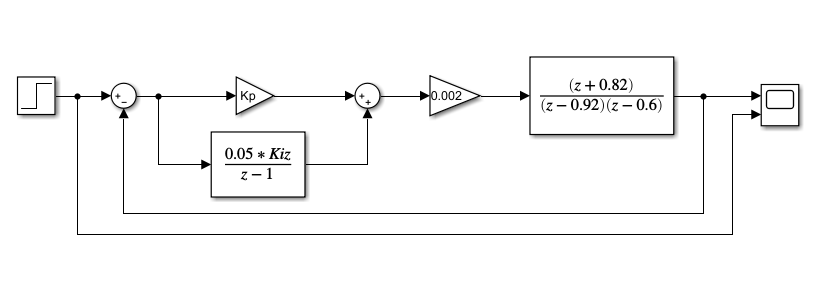
\includegraphics[width=0.9\columnwidth]{hw4-fig1.png}}
        \caption{Simulink Model for DC Motor}
        \label{fig: 1}
\end{figure}

\subsection{}
\begin{figure}[H]
    \centering
    \subfigure[$K_I=100, K_P=100 \quad and \quad \delta(t)=1$]{
        \textsf{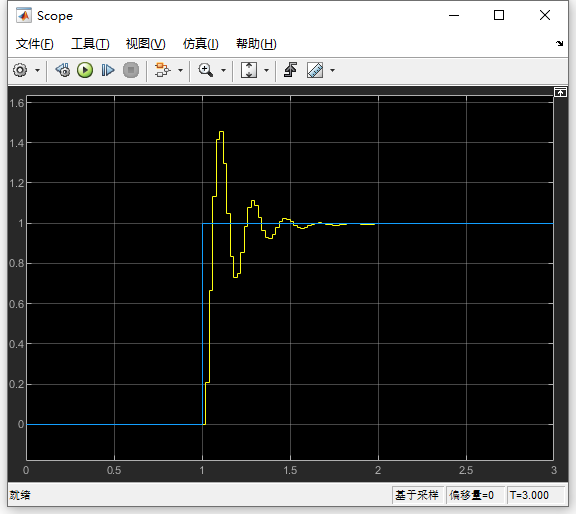
\includegraphics[width=0.4\columnwidth]{hw4-fig2.png}}
    }
    \quad
    \subfigure[Tracting Error for (a)]{
        \textsf{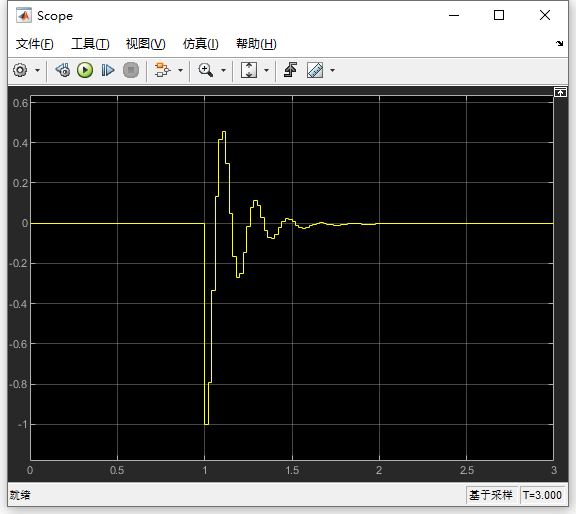
\includegraphics[width=0.4\columnwidth]{hw4-fig2-2.png}}
    }
    \quad
    \subfigure[$K_I=100, K_P=80 \quad and \quad \delta(t)=10$]{
        \textsf{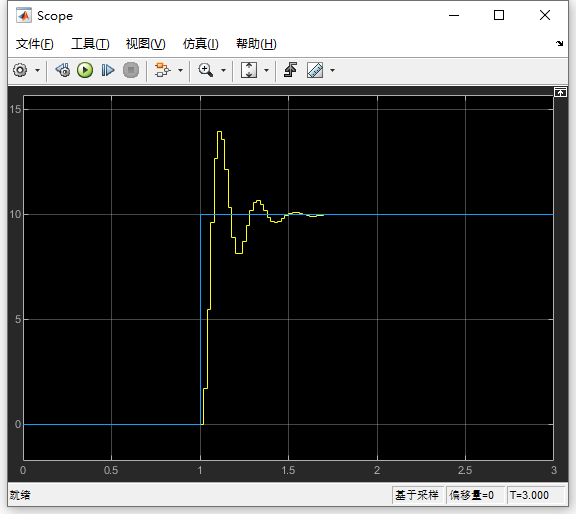
\includegraphics[width=0.4\columnwidth]{hw4-fig3.png}}
    }
    \quad
    \subfigure[Tracting Error for (b)]{
        \textsf{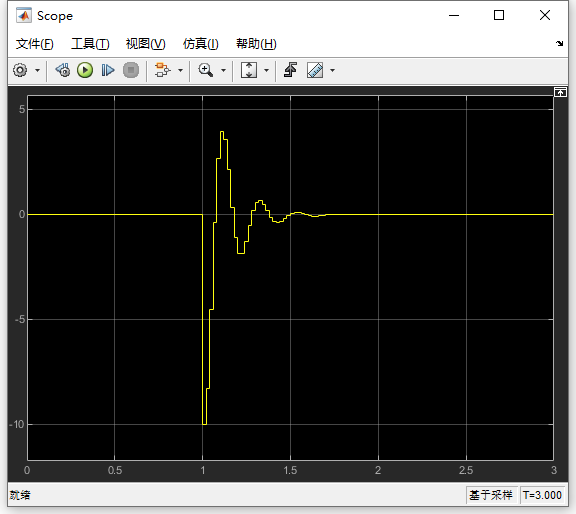
\includegraphics[width=0.4\columnwidth]{hw4-fig3-2.png}}
    }
    \caption{Simulation Results (T = 0.02)}
    \label{fig: 1}
\end{figure}
\subsection{}

For the first set:\\
Open loop transfer function is
$
G(z) = \frac{0.002(105z-100)(z+0.82)}{(z-1)(z-0.92)(z-0.6)}
$\\
By MATLAB, the closed loop poles are $0.99,0.66\pm0.53i$, which are all less than 1,
so the new system is BIBO stable.
\\On the other hand,
\begin{align*}
    e(\infty)&=\lim_{z\rightarrow1}(z-1)\frac{\frac{z}{z-1}}{1+G(z)}\\
    &= \lim_{z\rightarrow1}\frac{z(z-1)(z-0.92)(z+0.82)}{0.002(105z-100)(z+0.82)+(z-1)(z-0.92)(z+0.82)}\\
    &= 0
\end{align*}
For the second set, we have the same conditions for closed loop poles,
 and the steady state error $e(\infty)$ converge to 0 in a similar process as I showed above.
\end{document}
